\documentclass{article} % simplest latex class that gives nice default structures.  Other classes include standalone, book

% Recommended packages:
\usepackage{listings} % used for listing code

\usepackage{graphicx} % used for importing graphics


% Suggested packages:
\usepackage{tikz} % used for drawing figures in LaTeX directly
\usetikzlibrary{automata,calc,arrows} % some useful default tikz packages

\usepackage{enumerate} % used for finer control over enumerate lists

\usepackage{algorithm} % used for specifying algorithms
\usepackage{algpseudocode} % ditto (you need both)
\usepackage{amsmath}
\usepackage{fullpage} % reduces a page's margins to 1cm instead of 1in

\usepackage{mathpazo} % better? fonts

\usepackage{hyperref} % hyperlinks: compile with pdflatex for best results

\usepackage{amssymb}


\begin{document}

\title{Exam}
\author{Tianyi Zhu} % let's keep things anonymous
\maketitle % to actually insert the above three items

\section*{Question 1} % use section* to suppress numbering
\subsection*{(a)}
\subsubsection*{(i)}
$ f(x) = x\ div\ \left| x \right| $
\subsubsection*{(ii)}
$ g(x) = \left\lceil x \% 1 \right\rceil $
\subsubsection*{(iii)}
$ h(x) =  1 + \left\lfloor \left| x \right| \div 5 \right\rfloor - \left\lceil \left| x \right| \div 5 \right\rceil $
\subsubsection*{(iv)}
$ min(x,y) = (\left| x \ div \ y \right| div \left| x \ div \ y \right|) \times x + (\left| y \ div \ x \right| div \left| y \ div \ x \right|) \times y$
\subsubsection*{(v)}
$ q(x) = (g(x) + h(x))\ div \ 2 = (\left\lceil x \% 1 \right\rceil + 1 + \left\lfloor \left| x \right| \div 5 \right\rfloor - \left\lceil \left| x \right| \div 5 \right\rceil)\ div \ 2 $

\subsection*{(b)}
\subsubsection*{(i)}
Let $n = 10x + y$ where $x=\left\lfloor \frac{n}{10} \right\rfloor$ and $y = n \% 10$. Then $n' = x - 5y$ by definition.\\
$\because n|17$\\
$\therefore 5n|17$\\
$5n+n' = 50x+5y+x-5y = 51x = 17(3x)$\\
$\because x\in\mathbb{Z}$\\
$\therefore 5n+n'|17 $\\
Let $5n+n' = 17a$ and $5n = 17b$ where $a,b \in \mathbb{Z}$. Then $n' = 17(a-b)$\\
$\because a-b \in \mathbb{Z}$\\
$\therefore n'|17$
\subsubsection*{(ii)}
In some case like $n = 51$, $n'$ would never reach a negative value. So I replace negative with nonpositive in this question\\
By the definition of this rule, the number of digits in $n'$ must be at least 1 fewer than that in $n$. In the worst case, such as $n = 10$ and $n' = 1$, the number of digits only reduces by 1.\\
So we can only make sure $n'$ is nonpositive if $\left\lfloor \frac{n}{10} \right\rfloor = 0$, in other words, the number of digits in $n$ is 1.\\
The number of digits in $n$ is $log_{10}n + 1$ and it needs at most $log_{10}n + 1$ times of process to get a nonpositive $n'$.\\
Therefore the asymptotic upper bound is $O(logn)$\\
\section*{Question 2}
\subsection*{(a)}
\subsubsection*{(i)}
Let $X=\emptyset, A=\{1\}, B=\{2\}$. Then $A \cap X = \emptyset $ and $B \cap X = \emptyset $\\
$\because A \cap X = B \cap X$ and $A \neq B$\\
$\therefore (A \cap X = B \cap X) \not\to (A = B) $
\subsubsection*{(ii)}
\[
    \begin{array}{rll}
        A \oplus X  &=& (A \backslash X) \cup (X \backslash A)\\
                    &=& (A \cap X^c) \cup (X \cap A^c)\\
    \end{array}
\]
Similarly, $B \oplus X = (B \cap X^c) \cup (X \cap B^c)$\\
For some $a \in A \oplus X$, $a$ is either in $A \cap X^c$ or $X \cap A^c$\\
Because $A \oplus X = B \oplus X$, $a \in B \oplus X$. Then $a$ is either in $B \cap X^c$ or $X \cap B^c$\\
If $a \in A \cap X^c$, then $a \notin X$. So $a \notin X \cap B^c$ and $a \in B \cap X^c$\\
If $a \in X \cap A^c$, then $a \notin X^c$. So $a \notin B \cap X^c$ and $a \in X \cap B^c$\\
Therefore $A \cap X^c = B \cap X^c$ and $X \cap A^c = X \cap B^c$.\\
\\
Assume there is some $n \in A$ and $n \notin B$\\
If $n \in X$, then $n \in X \cap B^c$ and $n \notin X \cap A^c$. It is contradictory since $X \cap A^c = X \cap B^c$\\
If $n \notin X$, then $n \in A \cap X^c$ and $n \notin B\cap X^c$. It is contradictory since $A \cap X^c = B \cap X^c$\\
Therefore for all elements of $A$, it is an elements of $B$.\\
Hence $A \subseteq B$\\
\\
Assume there is some $m \in B$ and $n \notin A$\\
If $m \in X$, then $m \in X \cap A^c$ and $n \notin X \cap B^c$. It is contradictory since $X \cap A^c = X \cap B^c$\\
If $m \notin X$, then $m \in B \cap X^c$ and $n \notin A\cap X^c$. It is contradictory since $A \cap X^c = B \cap X^c$\\
Therefore for all elements of $B$, it is an elements of $A$.\\
Hence $B \subseteq A$\\
\\
Because $A \subseteq B$ and $B \subseteq A$, $A = B$.
\subsubsection*{(iii)}
$A \cap X = B \cap X$ and $A \cup X = B \cup X$\\
Assume there is some $n \in A$ and $n \notin B$, then $n \in A \cup X$ and $n \notin B \cup X$. So it is contradictory because $A \cup X = B \cup X$\\
Therefore for all elements of $A$, it is an elements of $B$.\\
Hence $A \subseteq B$\\
\\
Assume there is some $m \in B$ and $n \notin A$, then $m \in B \cup X$ and $n \notin A \cup X$. So it is contradictory because $A \cup X = B \cup X$\\
Therefore for all elements of $B$, it is an elements of $A$.\\
Hence $B \subseteq A$\\
\\
Because $A \subseteq B$ and $B \subseteq A$, $A = B$.
\subsection*{(b)}
\subsubsection*{(i)}

\subsubsection*{(ii)}
Let $\Sigma = \{0, 1\}, X = \{0, 1, 00, 01, 10, 11\}, Y =\{0, 1\}, Z=\{0, 1\}$\\
$\because X = Z \cup \{00,01,10,11\}$ and $Z^2 = \{00,01,10,11\}$\\
$\therefore X^*=Z^*$\\
$\because Z= \Sigma$\\
$\therefore X^*=Z^*=\Sigma $\\
$\because Y = \Sigma $\\
$\therefore X^*Y = YZ^* = \Sigma/\lambda$\\
$\because X^*Y = YZ^*$ while $XY \neq YZ$\\
$\therefore$ It is not necessary to be true.

\section*{Question 3}
Consider $A$ is not empty because $f$ is bijection if $A$ is an emptyset, and that conflicts with (c).
\subsection*{(a)}
\subsubsection*{$(a \preceq b) \to (f(a) \subseteq f(b))$}
Because $(A, \preceq)$ is a poset, $\preceq$ is reflexive, antisymmetric and transitive.\\
For all $c \preceq a$, we can get $c \preceq b$ by transitivity of $\preceq$ if $a \preceq b$.\\
So if $c \in \{x:x \leq a\}$, then $c \in \{x:x \leq b\}$. For each element in $f(a)$, it is an element of $f(b)$. \\
Therefore $f(a) \subseteq f(b)$

\subsubsection*{$ (f(a) \subseteq f(b)) \to (a \preceq b)$}
Becuase $f(a) = \{x:x \leq a\}$, $a \in f(a)$. $a\in f(b)$ since $f(a)\subseteq f(b)$\\
$f(b) = \{x:x \leq b\}$, so $a \preceq b$.

\subsection*{(b)}
Assume there exists some $c, d \in A$ such that $f(c) = f(d)$ and $c \neq d$.\\
By the definition of $f$, $f(c) = \{x:x\leq c\}$ and $f(d) = \{x:x \leq d\}$\\
If $c \neq d$, then either $c \gneq d$ or $c \lneq d$ would hold.\\
\subsubsection*{$c \gneq d$:}
$f(c) \neq f(d)$ because $c\in f(c)$ and $c \notin f(d)$. It is contradictory.
\subsubsection*{$c \lneq d$:}
$f(d) \neq f(c)$ because $d \in f(d)$ and $d \notin f(c)$. It is contradictory.\\
\\
Therefore, if $f(c)=f(d)$ then $c=d$. $f$ is injective.

\subsection*{(c)}
Because there is at least one element in $f(a)$ which is $a$ itself for all $a \in A$, there is no $a$ such that $f(a) = \emptyset$.\\
Therefore $f(a)$ is not surjective since $\emptyset \subseteq A$.

\subsection*{(d)}
$c \preceq a$ and $c \preceq b$ since $c=glb(a,b)$. $ f(c)\subseteq f(a)$ and $ f(c) \subseteq f(b) $ by (a). Hence $f(c) \subseteq f(a) \cap f(b)$\\
Because $f$ is injective and if $x\preceq y$ then $f(x) \subseteq f(y)$.\\
If $c=glb(a,b)$ in $(A, \preceq)$, then $f(c) = glb(f(a),f(b))$ in $(f(A),\subseteq)$.\\
In poset $(f(A), \subseteq)$, there is $glb(X,Y) = X \cap Y$.\ (by page 83 in Relation slide).\\
So $f(c) = f(a) \cap f(b)$


\section*{Question 4}
\subsection*{(a)}
A function is bijection iff it is both injective and surjective.\\
Define $f:(A \times B) \times C \to A \times (B \times C)$ as $f(((a, b),c)) = (a,(b,c))$\\
By the definition of $f$, there exists an inverse $g:A \times (B \times C) \to (A \times B) \times C$ as $g((a,(b,c))) = ((a, b),c)$
\subsubsection*{Injective}
Let $((a_1, b_1), c_1),((a_2, b_2), c_2)$ be any elements in $(A \times B) \times C$.\\
$((a_1, b_1), c_1) = g \circ f(((a_1, b_1), c_1)) = g \circ f(((a_2, b_2), c_2)) = ((a_1, b_1), c_1)$\\
$f(((a_1, b_1), c_1)) = f(((a_2, b_2), c_2)$ iff $((a_1, b_1), c_1)=((a_2, b_2), c_2)$\\
Hence $f$ is injective.
\subsubsection*{Surjective}
Suppose $((a_3, b_3), c_3)\in (A \times B) \times C$ and $(a_4,(b_4, c_4))\in A \times (B \times C)$ such that $ g( (a_4,(b_4, c_4))) = ((a_3, b_3), c_3)$.\\
$f\circ g((a_4,(b_4, c_4))) = f(((a_3, b_3), c_3)) = (a_4,(b_4, c_4))$\\
For every elements in $A \times (B \times C)$, it is mapped to at least one element in $(A \times B) \times C$\\
Hence $f$ is surjective.\\ 
\subsection*{(b)}
Let $P$ be $f:S \to T$ is injective and $Q$ be for all functions $g,h: U \to S: f\circ g= f\circ h$ implies $g = h$
\subsubsection*{$P \to Q$}
$f$ is injective, then if $f(x) = f(y)$ then $x = y$\\
For all $a \in U$, $f(g(a))= f(h(a))$ if $f\circ g = f\circ h$. That means $g(a) = h(a)$ for all $a \in U$.\\ 
The domain and co-domain of $g$ and $h$ is the same and for all $(a, g(a))\in g$, $(a, g(a))\in h$.\\
Therefore $g=h$ and $P \to Q$
\subsubsection*{$Q \to P$}
$g,h: U \to S: f\circ g= f\circ h$ implies $g = h$\\
Assume $f$ is not injective and there only exists one pair of $x, y \in S$ such that $x\neq y$ and $f(x) = f(y)$.\\
Assume there exists $a,b\in U$ such that $a\neq b$,$g(a) = x$, $g(b) = y$, $h(a) = y$ and $h(b) = x$.\\
In this case, $g\neq h$ although $f\circ g = f \circ h$.\\
Therefore $\neg P \to \neg Q$ then $Q \to P$
\subsubsection*{}
Hence it holds.
\subsection*{(c)}
\subsubsection*{(I)}
$n^3\sqrt{n} \in O(n^{\frac{7}{2}})$
\subsubsection*{(II)}
$n^3 log(n) \in O(n^3 log(n))$
\subsubsection*{(III)}
$T(n)$ where $T(0) = 1$ and $T(n) = T(n - 3) + n^3$\\
$T(n) = \left\lfloor \frac{n}{3}\right\rfloor \cdot n^3 + 1$\\
$T(n) \in O(n^4)$
\subsubsection*{(IV)}
$T(n)$ where $T(0) = 1$ and $T(n) = 6T(n/2) + n^3$\\
$a=6, b=2, c=3, d=log_b(a)=log_2(6)=2.58$\\
Because $c>d$, $T(n) \in O(n^3)$
\subsubsection*{(V)}
Because $O(log_n) \subseteq O(\sqrt{n})$, $O((3^{log \ n})^2) \subseteq O(3^{2\sqrt{n}})$\\
\subsubsection*{(VI)}
Because $O(log_n) \subseteq O(\sqrt{n})$, $O(3^{(log \ n)^2}) \subseteq O(3^{n})$\\
\subsubsection*{Conclusion}
$(IV)<(II)<(I)<(III)<(V)<(VI)$\\

\section*{Question 5}
Let's divided the code snippnet into 3 parts.\\
\begin{center}
    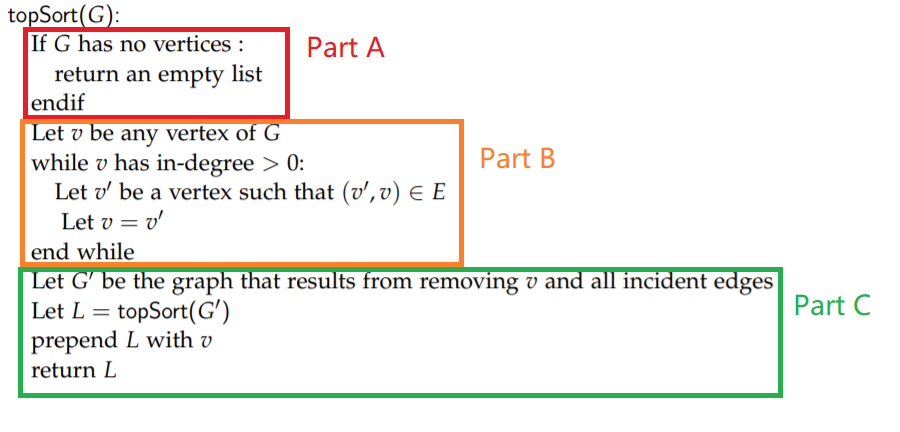
\includegraphics[scale = 0.5]{code 1.png}
\end{center}
\subsection*{(a)}
\subsubsection*{Part A}
.\quad If G has no vertices: \quad--$O(1)$\\
.\quad\quad return an empty list \quad--$O(1)$\\
.\quad endif\\
Assume this program check the size of matrix to find out whether it has vertices or not and it can be executed in $O(1)$ time.\\
Part A needs $O(1)$ time if $G$ has vertices and needs $2O(1)$ time if not.
So in the worst case, Part A needs $2O(1)$ to execute.
\subsubsection*{Part B}
.\quad Let $v$ be any vertex of $G$ \quad--$O(1)$\\
.\quad while $v$ has in-degree $> 0$: \quad--$O(n)$\\
.\quad\quad Let $v'$ be a vertex such that $(v', v) \in E$ \quad--$O(1)$\\
.\quad\quad Let $v = v'$ \quad--$O(1)$\\
.\quad endwhile\\
Because the matrix is not empty, there first column always exists. So let the 1st vertex be $v$ will spend $O(1)$ time.\\
To find out whether the in-degree of a vertices is 0 or not, the program needs to search in the corresponding column and check if all the number is 0.\\
In the worst case, the program needs to go through all the vertices in $G$ until it finds a vertice with 0 in-degree.\\ 
Go through all the vertices means search each column in the adjacency matrix and the while loop will be executed $n$ times.\\
So the running time Part B need is $O(n^2)+2O(n)+O(1)$
\subsubsection*{Part C}
Let $T(G(n))$ be the running time of $G$ and $O(G(n-i))$ be the running time of $G$ with $i$ vertices removed.\\
.\quad Let $G'$ be the graph that results from removing v and all incident edges\quad--$O(1)$\\
.\quad Let $L = topSort(G')$ \quad--$T(G(n-1))$\\
.\quad prepend $L$ with $v$ \quad--$O(1)$\\
.\quad return $L$ \quad--$O(1)$\\
Part C needs $T(G(n-1))+3O(1)$\\
\subsubsection*{Conclustion}
\[\begin{array}{rll}
    T(G(n)) &=&2O(1)+O(n^2)+2O(n)+O(1) +T(G(n-1)) +3O(1)\\
    T(G(n)) &=&T(G(n-1)) +O(n^2)+2O(n)+6O(1)\\
\end{array}\]
\[\begin{array}{rll}
    T(G(n))-T(G(n-1))   &=& O(n^2)+2O(n)+6O(1)\\
    T(G(n-1))-T(G(n-2)) &<& O(n^2)+2O(n)+6O(1)\\
    T(G(n-2))-T(G(n-3)) &<& O(n^2)+2O(n)+6O(1)\\
                    &......&\\
    T(G(1)) - T(G(0))   &<&  O(n^2) +2O(n) +6O(1)\\
    T(G(0))             &<& O(n^2) +2O(n) +6O(1)\\
\end{array}\]
Therefore $T(G(n)) = nO(n^2) + nO(n)+6nO(1) = O(n^3)$
\subsection*{(b)}
\subsubsection*{Part A}
Time cost in part A is the same as (a) which is $2O(1)$\\
\subsubsection*{Part B}
.\quad Let $v$ be any vertex of $G$ \quad--$O(1)$\\
.\quad while $v$ has in-degree $> 0$: \quad--$O(1)$\\
.\quad\quad Let $v'$ be a vertex such that $(v', v) \in E$ \quad--$O(m)$\\
.\quad\quad Let $v = v'$ \quad--$O(1)$\\
.\quad endwhile\\
To find out whether the in-degree of a vertices is 0 or not, the program needs to go through the whole list and check if this vertice never appears. This operation spends $O(m)$ time.\\
In the worst case, the program needs to go through all the vertices in $G$ until it finds a vertice with 0 in-degree. So the while loop need to be executed $n$ times\\ 
So the running time Part B need is $O(n*m)+2O(n)+O(1)$
\subsubsection*{Part C}
Time cost in part C is the same as (a) which is $T(G(n-1))+3O(1)$\\
\subsubsection*{Conclusion}
\[\begin{array}{rll}
    T(G(n)) &=&2O(1)+O(n*m)+2O(n)+O(1) +O(G(n-1)) +3O(1)\\
    T(G(n)) &=&T(G(n-1)) +O(n*m)+2O(n)+6O(1)\\
\end{array}\]
\[\begin{array}{rll}
    T(G(n)) &=& nO(m*n) + nO(n)+6nO(1) = O(m*n^2)\\
\end{array}\]
\subsection*{(c)}
\subsubsection*{Part A}
Time cost in part A is the same as (a) which is $2O(1)$\\
\subsubsection*{Part B}
.\quad Let $v$ be any vertex of $G$ \quad--$O(1)$\\
.\quad while $v$ has in-degree $> 0$: \quad--$O(m)$\\
.\quad\quad Let $v'$ be a vertex such that $(v', v) \in E$ \quad--$O(1)$\\
.\quad\quad Let $v = v'$ \quad--$O(1)$\\
.\quad endwhile\\
To find out whether the in-degree of a vertices is 0 or not, the program go through the corresponding row and check if there is no 1 in it .This operation spends $O(m)$ time.\\
In the worst case, the program needs to go through all the vertices in $G$ until it finds a vertice with 0 in-degree. So the while loop need to be executed $n$ times\\ 
So the running time Part B need is $O(n*m)+2O(n)+O(1)$
\subsubsection*{Part C}
Time cost in part C is the same as (a) which is $T(G(n-1))+3O(1)$\\
\subsubsection*{Conclusion}
\[\begin{array}{rll}
    T(G(n)) &=&2O(1)+O(n*m)+2O(n)+O(1) +O(G(n-1)) +3O(1)\\
    T(G(n)) &=&T(G(n-1)) +O(n*m)+2O(n)+6O(1)\\
\end{array}\]
\[\begin{array}{rll}
    T(G(n)) &=& nO(m*n) + nO(n)+6nO(1) = O(m*n^2)\\
\end{array}\]
\section*{Question 6}
\subsection*{(a)}
\subsubsection*{Base case:}
$height(\tau) = -1$
\subsubsection*{Recursive case:}
$height((T_{left}, T_{right})) = max(height(T_{left}, height(T_{right}))) + 1$

\subsection*{(b)}
\subsubsection*{Base case:}
$balanced(\tau) = 1$\\
$balanced((T_{left}, T_{right})) = 0$ if $\left| height(T_{left})-height(T_{right})\right|\gneq 1$
\subsubsection*{Recursive case:}
$balanced((T_{left}, T_{right})) = balanced(T_{left}) \cap balanced(T_{right})$
\subsection*{(c)}
\subsubsection*{Base case:}
\[\begin{array}{lrll}
    P(\tau):& count(\tau) &=& 0\\
    \\
            & 2^{height(\tau) + 1}-1 &=& 2^{-1+1}-1\\
                                    &&=& 0\\
                                    \\
            &   count(\tau) &\leq& 2^{height(\tau) + 1}-1\\
\end{array}\]
Hence $P(\tau)$ holds.\\
\subsubsection*{Inductive case:}
Let $P(T_{left})$ and $P(T_{right})$ holds, I will prove $P((T_{left},T_{right}))$ holds.\\
\[\begin{array}{rll}
    count((T_{left}, T_{right}))&=& count(T_{left}) + count(T_{right}) + 1\\
                                &\leq& 2^{height(T_{left})+1} -1 + 2^{height(T_{right}) +1} - 1 + 1\\
                                &\leq& 2^{height(T_{left})+1} + 2^{height(T_{right}) +1} - 1\\
\end{array}\]
Because $height((T_{left}, T_{right})) = max(height(T_{left}, height(T_{right}))) + 1$\\
\[\begin{array}{rll}
    2^{height(T_{left})+1} + 2^{height(T_{right}) +1} -1&\leq& 2 \times 2^{height((T_{left}, T_{right}))+1-1} -1\\
                                                        &\leq& 2^{height((T_{left}, T_{right}))+1} - 1\\
    \\
    count((T_{left}, T_{right}))&\leq& 2^{height((T_{left}, T_{right}))+1} - 1
\end{array}\]
Hence when $P(T_{left})$ and $P(T_{right})$, $P((T_{left},T_{right}))$ holds.
\subsubsection*{Conclusion}
By induction, $P(T)$ holds.\\
\subsection*{(d)}
\subsubsection*{Base case:}
$Q(\tau):balanced(\tau) = 1$\\
\[\begin{array}{rll}
    count(\tau) &=& 0\\
    \\
    2^{height(\tau)/2}-1&=& 2^{-1/2}-1\\
                        &=& -0.2928\\
    \\
    count(\tau) &\leq& 2^{height(\tau)/2}-1\\
\end{array}\]
\subsubsection*{Inductive case:}
Let $Q(T_{left})$ and $Q(T_{right})$ holds, I will prove $Q((T_{left},T_{right}))$ holds.\\
If $(T_{left},T_{right})$ is not balanced, then $Q((T_{left},T_{right}))$ holds.\\
If $(T_{left},T_{right})$ is balanced, then $\left| height(T_{left}) - height(T_{right}) \right| \leq 1$\\
\[\begin{array}{rll}
    count((T_{left}, T_{right}))&=&     count(T_{left}) + count(T_{right}) + 1\\
                                &\geq&  2^{\frac{height(T_{left})}{2}} - 1 + 2^{\frac{height(T_{right})}{2}} - 1 + 1\\
                                &\geq&  2^{\frac{height(T_{left})}{2}} + 2^{\frac{height(T_{right})}{2}} - 1\\
\end{array}\]
Because $\left| height(T_{left}) - height(T_{right}) \right| \leq 1$, $height(T_{left}) \geq height((T_{left},T_{right})) - 2$ and $height(T_{right}) \geq height((T_{left},T_{right})) - 1$.\\
\[\begin{array}{rll}
    2^{\frac{height(T_{left})}{2}} + 2^{\frac{height(T_{right})}{2}} - 1 &\geq&  2\times 2^{\frac{height((T_{left},T_{right})) - 2}{2}} - 1\\
                                                                        &\geq& 2^{\frac{height((T_{left},T_{right}))}{2}} - 1\\
                                                                        \\
    count((T_{left}, T_{right}))&\geq& 2^{\frac{height(T_{left})}{2}} + 2^{\frac{height(T_{right})}{2}} - 1\\
                                &\geq& 2^{\frac{height((T_{left},T_{right}))}{2}} - 1                                                         
\end{array}\]
Hence $Q((T_{left},T_{right}))$ holds when $Q(T_{left})$ and $Q(T_{right})$ holds
\subsubsection*{Conclusion:}
By induction, $Q(T)$ holds.\\
\section*{Question 7}
\subsection*{(a)}
\subsubsection*{(i)}
Let $R,O,G,B$ represents Red (Orange Green Blue) is a crewmate.\\
Premises:\\
\[\begin{array}{lrcl}
    \varphi_1: & R &\leftrightarrow& (R \cap B) \cup (\neg R\cap \neg B)\\
    \varphi_2: & O &\leftrightarrow& \neg R \cup \neg G\\
    \varphi_3: & G &\leftrightarrow& \neg R\\
    \varphi_4: & B &\leftrightarrow& \neg R\\
    \psi: &\varphi_1 \cap \varphi_2 &\cap& \varphi_3 \cap \varphi_4\\
\end{array}\]
The logical problem needs to be solved is that find the satisfying assignment for $\psi$\\
\subsubsection*{(ii)}
Truth table:\\
\begin{table}[h]
    \begin{tabular}{llll|llll|l}
            R & O & G & B & $\varphi_1$ &$\varphi_2$ & $\varphi_3$ & $\varphi_4$ & $\psi$ \\ \hline
            True  & True  & True  & True  & True  & False & False & False & False \\
            True  & True  & True  & False & False & False & False & True  & False \\
            True  & True  & False & True  & True  & True  & True  & False & False \\
            True  & True  & False & False & False & True  & True  & True  & False \\
            True  & False & True  & True  & True  & True  & False & False & False \\
            True  & False & True  & False & False & True  & False & True  & False \\
            True  & False & False & True  & True  & False & True  & False & False \\
            True  & False & False & False & False & False & True  & True  & False \\
            False & True  & True  & True  & True  & True  & True  & True  & True  \\
            False & True  & True  & False & False & True  & True  & False & False \\
            False & True  & False & True  & True  & True  & False & True  & False \\
            False & True  & False & False & False & True  & False & False & False \\
            False & False & True  & True  & True  & False & True  & True  & False \\
            False & False & True  & False & False & False & True  & False & False \\
            False & False & False & True  & True  & False & False & True  & False \\
            False & False & False & False & False & False & False & False & False
    \end{tabular}
\end{table}
\\
Red is an imposter when Orange, Green and Blue are crewmates.
\subsection*{(b)}
\subsubsection*{(i)}
Assume that there exist some $x$ such that $x = x'$\\
\[\begin{array}{rllr}
    x \vee x'&=& x \vee x\\
                &=& x &\quad\mbox{(Idempotence))}\\
                \\
    x \vee x' &=& 1 &\quad\mbox{(complementation)}\\
\end{array}\]
Hence $x = 1$. Because $1' = 0$ (by Assignment 3 Q1(1) and duality), $x'=0$ and $x'=x=1$.\\
Because of the uniqueness of complementation, $x'$ cannot has two different values.\\
Therefore there exists no $x$ such that $x=x'$.
\subsubsection*{(ii)}
RHS:
\[\begin{array}{rllr}
    (x \wedge y) \vee (x' \wedge z) &=& (x \wedge (y \wedge 1)) \vee (x' \wedge (z \wedge 1)) &\quad\mbox{(Identity)}\\
                                    &=& (x \wedge (y \wedge (z \vee z')))) \vee (x' \wedge (z \wedge (y \vee y')))) &\quad\mbox{(Complementation)}\\
                                    &=& (x \wedge ((y \wedge z)\vee(y \wedge z'))) \vee (x' \wedge ((z \wedge y) \vee (z \wedge y')) &\quad\mbox{(Distributivity)}\\
                                    &=& ( (x \wedge (y \wedge z)) \vee (x \wedge (y \wedge z')) )\vee ((x' \wedge (z \wedge y)) \vee (x' \wedge (z \wedge y')))&\quad\mbox{(Distributivity)}\\
                                    &=& ( (x \wedge (y \wedge z)) \vee (x \wedge (y \wedge z')) )\vee ((x' \wedge (y \wedge z)) \vee (x' \wedge (y' \wedge z)))&\quad\mbox{(Commutativity)}\\
                                    &=& ((x \wedge (y \wedge z)) \vee (x' \wedge (y \wedge z)) \vee ( (x' \wedge (y' \wedge z)) \vee (x \wedge (y \wedge z'))) &\quad\mbox{(Associativity)}\\
                                    &=& (((y \wedge z) \wedge x) \vee ((y \wedge z)\wedge x') \vee ( (x' \wedge (y' \wedge z)) \vee (x \wedge (y \wedge z'))) &\quad\mbox{(Commutativity)}\\
                                    &=& ((y \wedge z)\wedge(x \vee x')) \vee ( (x' \wedge (y' \wedge z)) \vee (x \wedge (y \wedge z')))&\quad\mbox{(Distributivity)}\\
                                    &=& ((y \wedge z)\wedge 1) \vee ( (x' \wedge (y' \wedge z)) \vee (x \wedge (y \wedge z')))&\quad\mbox{(Complementation)}\\
                                    &=& (y \wedge z) \vee ( (x' \wedge (y' \wedge z)) \vee (x \wedge (y \wedge z')))&\quad\mbox{(Identity)}\\
                                    \\
    (x \wedge y) \vee (x' \wedge z) &=& ((y \wedge z)\vee(y \wedge z)) \vee ( (x' \wedge (y' \wedge z)) \vee (x \wedge (y \wedge z')))&\quad\mbox{(Absorption)}\\
                                    &=& (y \wedge z)\vee((y \wedge z) \vee ( (x' \wedge (y' \wedge z)) \vee (x \wedge (y \wedge z')))) &\quad\mbox{(Associativity)}\\
                                    &=& (y \wedge z)\vee ((x \wedge y) \vee (x' \wedge z)) &\quad\mbox{(By the result above)}\\
                                    &=& ((x \wedge y) \vee (x' \wedge z)) \vee (y \wedge z) &\quad\mbox{(Associativity)}
\end{array}\]
RHS = LHS, so it holds.
\section*{Question 8}
\subsection*{(a)}
If there exists Eulerian circuit in $G$, then every time we arrive at a vertex during our traversal of $G$, we can enter via one edge and exit via another.\\
So if we can reach a vertex, it must has another edge for exiting.\\
\subsubsection*{Undirection graph}
$G$ has an Eulerian circuit iff $deg(v)$ is even for all $v \in V$. \\
Because the vertex with odd degree can only be either the start vertex or end vertex in Eulerian path.\\
\subsubsection*{Direction graph}
$G$ has an Eulerian circuit iff $indeg(v) = outdeg(v)$ for all $v\in V$.\\
Because the vertex with $indeg(v) \neq outdeg(v)$ can only be either the start vertex or end vertex in Eulerian path.\\
\subsection*{(b)}
\subsubsection*{Undirection graph}
The number of edges in $G$ is $\frac{1}{2} \sum_{v\in V}deg(v)$.\\
Because there exists an Eulerian circuit, $deg(v)$ is even for all $v \in V$.\\
Because number of vertices is even and $deg(v)$ is even for all $v \in V$, the number of edges is a product of an even number which is always even.\\
Therefore the number of edges is even.
\subsubsection*{Direction graph}
The number of edges in $G$ is the $\sum_{v\in V}(indeg(v) + outdeg(v))$\\
Because there exists an Eulerian circuit, $indeg(v) = outdeg(v)$ for all $v\in V$.\\
So $(indeg(v) + outdeg(v)$ is even for all $v \in V$\\
Therefore the number of edges is even.
\subsection*{(c)}
Because $G$ is bipartite, the chromatic number is at most 2.\\
\subsection*{(d)}
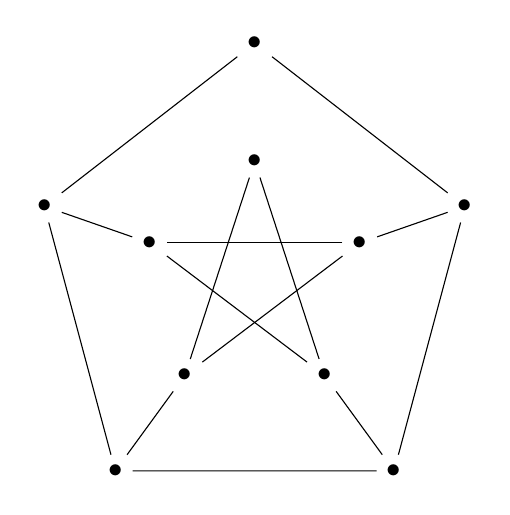
\begin{tikzpicture}[scale=1.5]
    \node (A) at (0,	2) {$\bullet$};
    \node (B) at (-1.78,	0.62) {$\bullet$};
    \node (C) at (-1.18,	-1.62) {$\bullet$};
    \node (D) at (1.18, -1.62) {$\bullet$};
    \node (E) at (1.78,	0.62) {$\bullet$};
    
    \node (AA) at (0,	1) {$\bullet$};
    \node (BB) at (-.89,	0.31) {$\bullet$};
    \node (CC) at (-0.59,	-0.81) {$\bullet$};
    \node (DD) at (0.59, -0.81) {$\bullet$};
    \node (EE) at (.89,	0.31) {$\bullet$};
    \path
    (A) edge (B)
    (B) edge (C)
    (C) edge (D)
    (D) edge (E)
    (E) edge (A)
    (B) edge (BB)
    (C) edge (CC)
    (D) edge (DD)
    (E) edge (EE)
    (AA) edge (CC)
    (CC) edge (EE)
    (EE) edge (BB)
    (BB) edge (DD)
    (DD) edge (AA);
    \end{tikzpicture}
    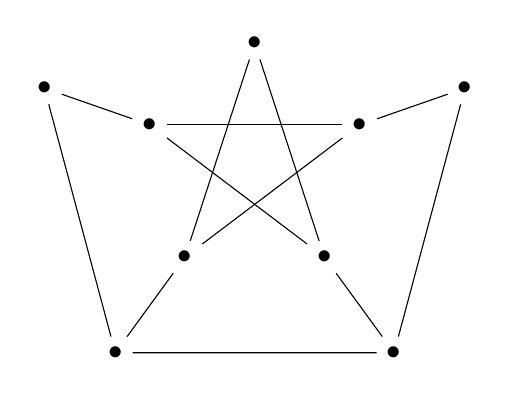
\begin{tikzpicture}[scale=1.5]
        \node (B) at (-1.78,	0.62) {$\bullet$};
        \node (C) at (-1.18,	-1.62) {$\bullet$};
        \node (D) at (1.18, -1.62) {$\bullet$};
        \node (E) at (1.78,	0.62) {$\bullet$};
        
        \node (AA) at (0,	1) {$\bullet$};
        \node (BB) at (-.89,	0.31) {$\bullet$};
        \node (CC) at (-0.59,	-0.81) {$\bullet$};
        \node (DD) at (0.59, -0.81) {$\bullet$};
        \node (EE) at (.89,	0.31) {$\bullet$};
        \path
        (B) edge (C)
        (C) edge (D)
        (D) edge (E)
        (B) edge (BB)
        (C) edge (CC)
        (D) edge (DD)
        (E) edge (EE)
        (AA) edge (CC)
        (CC) edge (EE)
        (EE) edge (BB)
        (BB) edge (DD)
        (DD) edge (AA);
        \end{tikzpicture}
        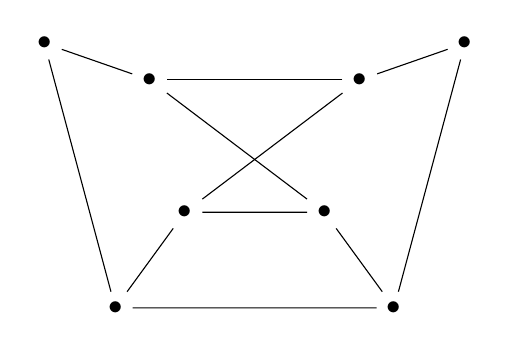
\begin{tikzpicture}[scale=1.5]
            \node (B) at (-1.78,	0.62) {$\bullet$};
            \node (C) at (-1.18,	-1.62) {$\bullet$};
            \node (D) at (1.18, -1.62) {$\bullet$};
            \node (E) at (1.78,	0.62) {$\bullet$};
            
            \node (BB) at (-.89,	0.31) {$\bullet$};
            \node (CC) at (-0.59,	-0.81) {$\bullet$};
            \node (DD) at (0.59, -0.81) {$\bullet$};
            \node (EE) at (.89,	0.31) {$\bullet$};
            \path
            (B) edge (C)
            (C) edge (D)
            (D) edge (E)
            (B) edge (BB)
            (C) edge (CC)
            (D) edge (DD)
            (E) edge (EE)
            (CC) edge (EE)
            (EE) edge (BB)
            (BB) edge (DD)
            (DD) edge (CC);
            \end{tikzpicture}
            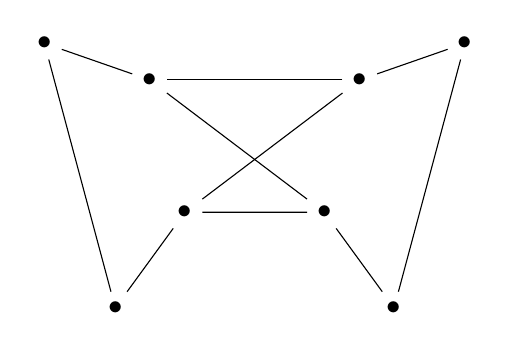
\begin{tikzpicture}[scale=1.5]
                \node (B) at (-1.78,	0.62) {$\bullet$};
                \node (C) at (-1.18,	-1.62) {$\bullet$};
                \node (D) at (1.18, -1.62) {$\bullet$};
                \node (E) at (1.78,	0.62) {$\bullet$};
                
                \node (BB) at (-.89,	0.31) {$\bullet$};
                \node (CC) at (-0.59,	-0.81) {$\bullet$};
                \node (DD) at (0.59, -0.81) {$\bullet$};
                \node (EE) at (.89,	0.31) {$\bullet$};
                \path
                (B) edge (C)
                (D) edge (E)
                (B) edge (BB)
                (C) edge (CC)
                (D) edge (DD)
                (E) edge (EE)
                (CC) edge (EE)
                (EE) edge (BB)
                (BB) edge (DD)
                (DD) edge (CC);
                \end{tikzpicture}
                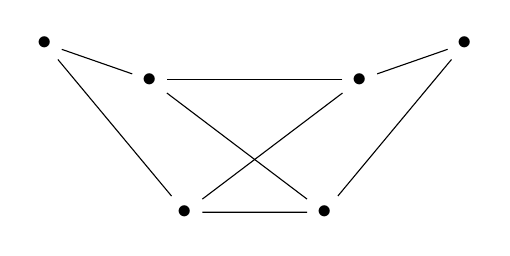
\begin{tikzpicture}[scale=1.5]
                    \node (B) at (-1.78,	0.62) {$\bullet$};
                    \node (E) at (1.78,	0.62) {$\bullet$};
                    \node (BB) at (-.89,	0.31) {$\bullet$};
                    \node (CC) at (-0.59,	-0.81) {$\bullet$};
                    \node (DD) at (0.59, -0.81) {$\bullet$};
                    \node (EE) at (.89,	0.31) {$\bullet$};
                    \path
                    (B) edge (BB)
                    (B) edge (CC)
                    (E) edge (DD)
                    (E) edge (EE)
                    (CC) edge (EE)
                    (EE) edge (BB)
                    (BB) edge (DD)
                    (DD) edge (CC);
                    \end{tikzpicture}
                    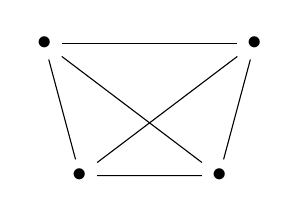
\begin{tikzpicture}[scale=1.5]
                        \node (BB) at (-.89,	0.31) {$\bullet$};
                        \node (CC) at (-0.59,	-0.81) {$\bullet$};
                        \node (DD) at (0.59, -0.81) {$\bullet$};
                        \node (EE) at (.89,	0.31) {$\bullet$};
                        \path
                        (CC) edge (BB)
                        (EE) edge (DD)
                        (CC) edge (EE)
                        (EE) edge (BB)
                        (BB) edge (DD)
                        (DD) edge (CC);
                        \end{tikzpicture}
\\
Therefore this graph contains a subdivision of $K_4$.
\subsection*{(e)}
$K_{4,4}$ is nonplanar because $4>3$.\\
$K_{2,16}$ is the same as $K_{16,2}$ and $K_{16,2}$ is planar.(By graph slide page108)\\
If graph $G$ contains, as a subgraph, a nonplanar graph, then $G$ itself is nonplanar. So if $K_{2,16}$ contain a subdivision of $K_{4,4}$, then $K_{2,16}$ is nonplanar.\\
Therefore $K_{2,16}$ does not contain a subdivision of $K_{4,4}$.\\
\section*{Question 9}
\subsection*{(a)}
For every $x \in A_n$, there must exist at least one $y\in A_n$ such that $x$ is mapped to $y$ by the definition of surjective.\\
For every $x \in A_n$, there must exist at least one $f(x)\in A_n$.\\
Because the size of domain and co-domain is both $n$, this function must be bijective.\\
So $F(n,n) = n!$\\
\subsection*{(b)}
For $n < 2$, there are 0 function which is surjective.\\
For every $x \in A_n$, there must exist at least one $y\in A_n$ such that $x$ is mapped to $y$ by the definition of surjective.\\
Select 2 elements in $A_n$ mapping to each $A_2$. The number of different ways to select is $\binom{n}{2}$ and the number of different orders is $2!$.\\
The rest of elements in $A_n$ can mapping to $A_2$ without limit. There are $\binom{2}{1}^{n-2}$ ways to select\\
There are 2 different elements in $A_2$. So $F(n,2) = 2!\binom{n}{2}2^{n-2}$\\
\subsection*{(c)}
Because two equivalent relations are different if their partitions of $A_n$ is different.\\
$E(n)$ is equal to the number of partitions of $A_n$ into equivalence classes.\\
It is similar to ask how many ways to place $n$ distinguishable balls in $n$ undistinguishable box.\\ 
\subsubsection*{[B]}
$E(1) = 1$
\subsubsection*{[R]}
If add $\{n\}$ to every equivalence class in $E(n)$, we can get $E(n)$ kinds of different equivalence class. (For example, the equivalence class of E(1) is $\{{1}\}$. Then add $\{2\}$ to it and we get $\{\{1\},\{2\}\}$)\\
$E(n+1) = E(n)+$
\subsection*{(d)}
\subsubsection*{Base case}
$F(0,k) = 0$\\
$F(n,0) = 1$\\
\subsection*{Recursive case}

\subsection*{(e)}
(Reference: https://math.stackexchange.com/questions/703475/determine-the-number-of-equivalence-relations-on-the-set-1-2-3-4)
If add $\{n\}$ to every equivalence class in $E(n-1,k-1)$, we can get $E(n-1,k-1)$ kinds of different equivalence class.\\
All equivalence relations by adjoining the nth element to one of the equivalence classes of a relation with $k$ equivalence classes in the remaining $n -1$ elements.\\
$E_{n,k} = E_{n-1, k-1}+kE_{n-1,k}$
\section*{Question 10}
\subsection*{(a)}
\[\begin{array}{rlll}
    P(A)    &=& P((A\backslash B) \cup (A \cap B)) &\quad\mbox{(Definition of /)}\\
            &=& P(A\backslash B) + P(A \cap B) - P((A \backslash B) \cap (A \cap B))   &\quad\mbox{(Inclusion-exclusion rule)}\\
            &=& P(A\backslash B) + P(A \cap B)\\
            \\
    P(B)    &=& P((B \backslash A) \cup (A \cap B))         &\quad\mbox{(Definition of /)}\\
            &=& P(B \backslash A) + P(A \cap B) - P((B \backslash A) \cap (A \cap B)) &\quad\mbox{(Inclusion-exclusion rule)}\\
            &=& P(B \backslash A) + P(A \cap B)\\
            \\
    P(A) - P(B) &=& P(A \backslash B) + P(A \cap B) - P(B\backslash A) - P(A \cap B)\\
                &=& P(A \backslash B) - P(B \backslash A)\\
\end{array}\]
$\because P(B \backslash A) \geq 0$\\
$\therefore P(A \backslash B) \geq P(A \backslash B) - P(B \backslash A)$\\
$\because P(A) - P(B) = P(A \backslash B) - P(B \backslash A)$\\
$\therefore P(A\backslash B) \geq P(A) - P(B)$
\subsection*{(b)}
\[\begin{array}{rlll}
    P(A|B) &=& \frac{P(A \cap B)}{P(B)} &\quad\mbox{(Definition of conditional probability)}\\
    \\
    P(B|A) &=& \frac{P(A \cap B)}{P(A)} &\quad\mbox{(Definition of conditional probability)}\\
\end{array}\]
$\because 0<P(A)\leq P(B)$\\
$\therefore \frac{1}{P(A)} \geq \frac{1}{P(B)}$\\
$\because \frac{1}{P(A)} \geq \frac{1}{P(B)}, P(A|B) = \frac{P(A \cap B)}{P(B)}$ and $P(B|A) = \frac{P(A \cap B)}{P(A)}$\\
$\therefore P(A|B) \leq P(B|A)$
\subsection*{(c)}
Assume $P(X = -1) = \frac{1}{3}, P(X = 0) = \frac{1}{3}, P(X = 1) = \frac{1}{3}$\\
\[\begin{array}{rll}
    E(X)    &=& -1\times P(X=-1) + 0\times P(X=0) + 1\times P(X=1) \\
            &=& -1\times \frac{1}{3} + 0 \times \frac{1}{3} + 1\times \frac{1}{3}\\
            &=& 0\\

\end{array}\]
$E(X) = -1\times P(X=-1) + 0\times P(X=0) + 1\times P(X=1) = 0$\\
$P(X>E(X)) = \frac{1}{3} <\frac{1}{2}$\\
$P(X > E(X))\geq \frac{1}{2}$ does not always hold.\\
\subsection*{(d)}
Assume $Y=X$ if $X$ exists. if else, $Y=0$. P($X$ exists) = $\frac{1}{2}$, $P(X=1) = \frac{1}{2}$, $P(X=2) = \frac{1}{2}$\\
\[\begin{array}{rll}
    E(Y)    &=& 0\times P(Y=0) + 1\times P(Y=1) + 2\times P(Y=2) \\
            &=& 0\times \frac{1}{2} + 1 \times \frac{1}{4} + 2\times \frac{1}{4}\\
            &=& \frac{3}{4}\\
            \\
    E(X)    &=& 1\times P(X=1) + 2\times P(X=2)\\
            &=& 1\times \frac{1}{2} + 2\times \frac{1}{2}\\
            &=& \frac{3}{2}
\end{array}\]
$P(X>Y) = 0$\\
Because $E(X) > E(Y)$ and $P(X>Y)\not> 0$, it does not always hold. If the selection of X value and Y value is independent to each other, it holds because the maximum of $X$ is greater than the minimum of $Y$.\\
\end{document}
